\section{Introduction}

%\subsection{Variable assignment}

%\subsection{Variable assignment}

\begin{frame}[fragile]
\frametitle{Variable assignment}

    Python is a dynamical binding and typing language, contrary to C/C++, Java and Fortran (source: \href{https://pythonconquerstheuniverse.wordpress.com/2009/10/03/static-vs-dynamic-typing-of-programming-languages/}{pythonconquerstheuniverse})

    \begin{center}
    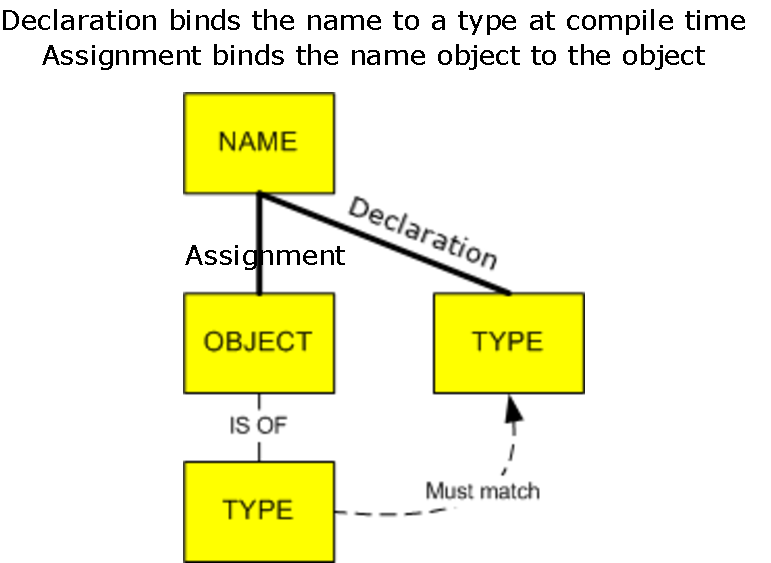
\includegraphics[scale=0.4]{figs/static_typing.pdf}
    %\hspace{1em}
    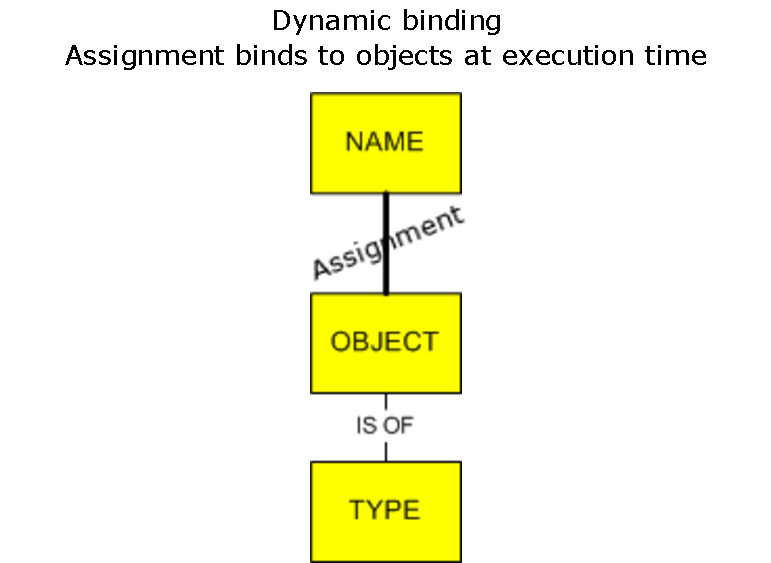
\includegraphics[scale=0.4]{figs/dynamic_typing.pdf}
    \end{center}

    Therefore, one variable name can be reused for different objects. Variable assignment is done with the \verb+=+ sign:
    \lstinputlisting[linerange={1-3}, basicstyle=\ttfamily\scriptsize]{scripts/vars.py}

\end{frame}


\begin{frame}[fragile]
    \frametitle{Variables as objects}

    Python is object oriented. Therefore, each assigned variable is an object, about which informations are accessible via:
    \lstinputlisting[linerange={4-6}, basicstyle=\ttfamily\scriptsize]{scripts/vars.py}

    \vspace{1em}
    Calling an object's method is done as follows:
    \lstinputlisting[linerange={8-10}, basicstyle=\ttfamily\scriptsize]{scripts/vars.py}

    \vspace{1em}
    To convert an object to another type:
    \lstinputlisting[linerange={12-12}, basicstyle=\ttfamily\scriptsize]{scripts/vars.py}

\end{frame}
    
\begin{frame}[fragile]
    \frametitle{Object's types}

    There are of \textbf{two} main caterogies of objects: (source: \href{https://www.geeksforgeeks.org/mutable-vs-immutable-objects-in-python/}{geeksforgeeks}): \\
    \begin{itemize}
        \item{\emph{Mutable objects}: Can't change their state and contents: \textbf{list, dict, set and custom objects (numpy.arrays for instance)}}
        \item{\emph{Immutable objects}: Can change their state and contents: \textbf{int, float, bool, string, unicode, tuple}}
    \end{itemize}

    \vspace{1em}
    For instance, the following statement will raise an error:
    \lstinputlisting[linerange={14-15}, basicstyle=\ttfamily\scriptsize]{scripts/vars.py}

    since string are immutable.

\end{frame}
